%!TEX root = /Users/smsohan/Taggy/Thesis/ucalgthes1_root_0.tex
\fancyhead[RO,LE]{\thepage}
\fancyfoot{} 
\chapter{Quantitative Evaluation}
\label{ch:evaluation}
As previously mentioned in the research goals, an evaluation is required to measure the accuracy of Taggy in auto-tagging emails with user stories. In this thesis, the evaluation is based on two different real world data sets, collected from two different sources. In total the data represents 4,745 messages created by 9 agile teams. The evaluation shows that for different projects Taggy can correctly auto-tag between 76\% emails with user stories after sufficient training.

This chapter is organized as follows: Firstly, the evaluation approach is discussed. As a part of it, the adapted definition of accuracy is given. Next, a null hypothesis is stated which is used in deducing the statistical relevance of the evaluation results. Then, the two data sets are described and the evaluation results for each are provided in detail. Finally, the limitations of this evaluation are discussed.

\section{Evaluation Approach}
The evaluation steps, as depicted in Figure~\ref{fig:evaluation}, are described below.

\begin{figure*}[h!]
	\centering
	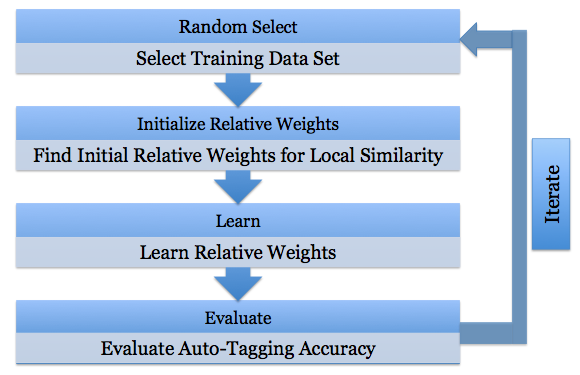
\includegraphics[width=\textwidth]{Evaluation.png}
	\label{fig:evaluation}
  \caption{Taggy Empirical Evaluation Steps}
\end{figure*}


\begin{enumerate}
	\item \textbf{Random Select.} Randomly select 10\% emails from all available emails for training. Training emails are randomly selected to improve the possibility of encountering different patterns in the data.
	\item \textbf{Initialize Relative Weights.} Initialize the relative weights for temporal, people, subject and body similarities using the training data from step\# 1.
	\item \textbf{Learn.} Use the reward-punishment approach for each training email from step\# 1, adjust the relative weights.
	\item \textbf{Evaluate.} Using the adjusted relative weights from step\#3, auto-tag the remaining emails that were not included in the training data in step\# 1. This ensures the training data and evaluation data contain completely disjoint sets of emails. Compute the accuracy of the auto-tagging.
	\item \textbf{Iterate.} Repeat steps 1 to 4, with 20\%, 30\%, 40\% and 50\% data for training. This step attempts to find an optimum partition of  training data set where the relative weights converge to a point so that adding more training data adds little value to the auto-tagging accuracy.
	
\end{enumerate}

\subsection{Accuracy}
The accuracy of auto-tagging is a ratio between the number of correct tags and the total number of emails presented for evaluation. Since this excludes the training data set, the accuracy only represents the accuracy over the evaluation data set. So, the accuracy is computed using Equation~\ref{eq:accuracy}.
	
\begin{equation}
\label{eq:accuracy}
Accuracy = \frac{Number \;  of  \; correct  \; auto tagging} {Number \;  of \;  total \;  evaluation \;  emails }  \; *  \; 100  \; \%
\end{equation}
	
As Equation~\ref{eq:accuracy} suggests, it is necessary to be able to justify whether an auto-tagging is correct or incorrect. So, the evaluation data needs to provide information about correct relationship of an email with user stories so that the auto-tagged results can be compared against  known values.

\subsection{Statistical Relevance}
The statistical relevance is found by starting with a null hypothesis and then observing the goodness-of-fit of the evaluation data based on chi-square test \cite{chi_square}. In this case the null hypothesis is:

\begin{quote}
	The auto-tagging accuracy of Taggy is no better than a random decision making.
\end{quote}

The outcome of an auto-tagging process is either a correct or a wrong tagging of an email against the user stories in a project. Similarly, a random system will produce one of the two outcomes. The target of this statistical relevance determination is to see if the accuracy found from Taggy's evaluation is likely to be achievable by a random system.

In this case, we have a single degree of freedom, since there are two possible outcomes, correct and incorrect. And the expected value of correct and incorrect decisions is same for a random system. Based on this information, the chi-square computation is done using Equation~\ref{eq:chi}:

\begin{equation}
\label{eq:chi}
\begin{split}
	\chi ^ 2 = \frac {(Count \; of \; correct \; tagging \; - \; half \; of \; total \; evaluation \; emails) ^ 2} {half of total evaluation emails} +  	
\\
	\frac{(Count \; of \; wrong \; tagging \; - \; half \; of \; total \; evaluation \; emails)  ^ 2} {half \; of \; total \; evaluation \; emails}
\end{split}	
\end{equation}                                       

This computed $\chi^{2}$ value is compared against the upper critical chi-square value for probability 0.05 with 1 degree of freedom, that is $\chi^{2}_{0.05}$=3.841. The probability value of 0.05 is conventionally used in significance finding. A value beyond this threshold indicates disagreement between the observation and the null hypothesis. We also present the corresponding p-values against the computed chi-square values. The lower the p-value, the less likely it is that the observation given the null hypothesis is true.

\section{Evaluation Results}
The evaluation results are discussed in two sections for two different data sets.

\subsection{Data set\# 1: ScrumPad}	
This data set was obtained from an online agile project management tool called ScrumPad.	ScrumPad allows users to manage product backlog, perform iteration planning and track progress. Also, it lets users discuss the project's user stories using message threads. Each message thread can contain an explicit link to a user story. While sending a message using ScrumPad, one can link it with a user story. The messages are stored in ScrumPad database and also sent to people via emails. People can directly reply to the notification emails, which goes to ScrumPad and gets saved as a message either in a new or under an existing thread.

The user stories in ScrumPad contain information about its title, description, attachments, customer, developers and iteration. Taggy used these user stories to train and evaluate its auto-tagging performance.

\begin{figure*}[h!]
	\centering
	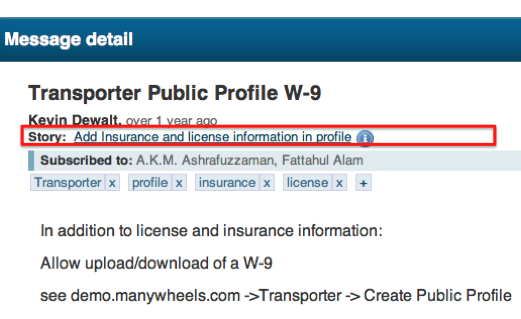
\includegraphics[width=0.8\textwidth]{scrumpad_message.png}
   \caption{A ScrumPad Message Linked to a User Story}
	\label{fig:scrumpad_message}
\end{figure*}

Figure~\ref{fig:scrumpad_message} shows the screenshot of a message at ScrumPad. As this figure shows, the message has a link to the user story. The messages from ScrumPad message threads are derived as emails for the evaluation of Taggy. Messages contain subject, body, sender, recipients and attachments. These fields are mapped against the standard fields of emails. Also, if a message thread in ScrumPad is linked against a user story, all derived emails from the messages of that thread are also treated to be linked against the user story. So, these are essentially the correct tags for the emails since they were all manually provided by the contributors to the message threads. This information helps the training of Taggy using reward-punishment approach with the necessary feedback. Also, the accuracy computation relies on this information to find if an auto-tagging is correct or not.

ScrumPad data set contains data from five distributed agile projects. Four of the five projects, MethodMarketing, BI for Car Dealers, ManyWheels and VarsityDays were developed by Code71, Inc. (www.Code71.com). Code71 is also the creator of ScrumPad. These four projects employed developers from Dhaka, Bangladesh and Virginia, USA. These projects were developed for four different clients from USA.

The fifth project, MindAndMarket, was distributed among one developer from Bangladesh, and two developers and a client from Belgium. The Belgian development team and the client worked at the same city.

\begin{table}[h!]
  \centering
  \caption{Scrumpad Data Set}
	\label{tab:scrumpad_data_set}
    \begin{tabular}{|p{2cm}|p{4cm}|r|p{1cm}|p{1.2cm}|p{1.2cm}|r|}
      \hline
      \textbf{Project Name} & \textbf{Description} & \textbf{Users} & \textbf{Itera- tions} & \textbf{It. Len. (days)}  & \textbf{User Stories} & \textbf{Emails}\\
      \hline
      Method Marketing & Online loan application & 7 & 14 & 14 & 86 & 183 \\
      \hline
      BI for Car Dealers & A decision support tool for vehicle dealers & 7 & 11 & 14 & 70 & 213 \\
      \hline
      Many Wheels & A web application for transporters and shippers & 5 & 12 & 14 & 97 & 158 \\
      \hline
      Varsity Days & A social networking application for school sports teams & 5 & 15 & 14 & 88 & 46 \\
      \hline
      Mind And Market & A project collaboration tool & 3 & 6 & 7 & 28 & 40 \\
      \hline
      \textbf{Total} &  &  &  &  & \textbf{369} & \textbf{640}\\
      \hline
    \end{tabular}
\end{table}

Table~\ref{tab:scrumpad_data_set} shows the composition of this data set. In total, this data set contained 640 emails and 369 user stories from 5 distributed agile projects. It is worth mentioning that 640 messages were exchanged using ScrumPad. However, the actual number of project related emails may not be limited to this volume.

Given this data, the aforementioned evaluation approach was followed to train and auto-tag the emails. The iterative approach resulted in an optimum  training data partition size of 20\%. This size was selected because, a random partition containing 20\% of all emails for training produced better auto-tagging accuracy than a smaller sized partition (e.g. 10\%) and was as good as a larger sized partition (e.g. 30\%). 

\begin{figure*}[htb]
	\centering
	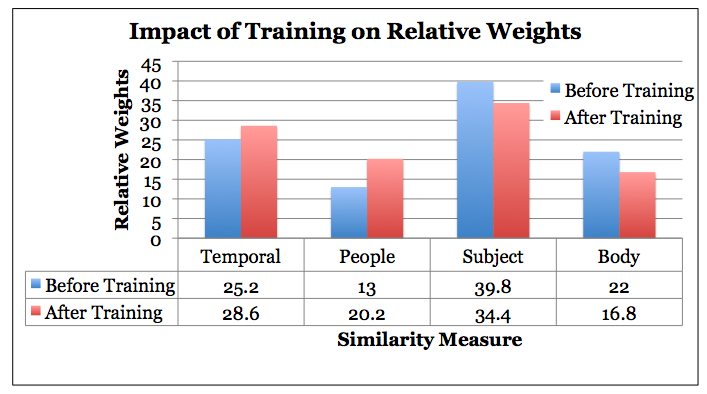
\includegraphics[width=\textwidth]{training.png}
    \caption{Impact of Training on Relative Weights}
	\label{fig:training}
\end{figure*}

Chart~\ref{fig:training} shows the impact of training on the relative weights of different similarity measures. The chart shows that the initial relative weights for the similarity measures of the text components (subject and body) are reduced while the context components (temporal and people) are increased as a result of the training.

Instead of training Taggy on a per project basis, I used 20\% data from all the projects. As a result, Taggy could benefit from a large number of training emails. However, it is possible to use a per project learning as well. I have discussed the trade-off regarding learning for specific project vs. a collection of projects at Chapter~\ref{ch:discussion}.

The maximum similarity score for a local similarity measure can be 1.0 as shown in the similarity equations at Section~\ref{sec:equations}. Using the trained relative weight values and a threshold global similarity score of 0.58, an email will be auto-tagged with a user story if one of the following is true:
\begin{enumerate}
	\item The email has strong text similarity (maximum 0.34 + 0.17 ~= 0.51) and some context similarity with the user story.
	\item The email has context similarity (maximum 0.29 + 0.20 ~= 0.49) and some text similarity with the user story.
\end{enumerate}
So, setting such a threshold score forces auto-tagging decisions to be based on both context and text relevance. This threshold was found from observing the data. In the training data, the global similarity function produced a score of 0.58 or higher for 90\% of the actual email and user story relations. This cut-off point helped to eliminate some false positives and false negatives. The trade-off between selecting this threshold and auto-tagging is discussed later in Chapter~\ref{ch:discussion}.  

Using this threshold and the trained relative weights, the evaluation yielded the results as shown in Table~\ref{tab:sp_evaluation}.

\begin{table}[h!]
  \centering
  \caption{Evaluation Using Scrumpad Data Set}
	\label{tab:sp_evaluation}
    \begin{tabular}{|p{2cm}|p{2cm}|p{2cm}|p{2cm}|p{2cm}|p{2cm}|p{1.5cm}|p{1.5cm}|}
      \hline
      \textbf{Project Name} & \textbf{Total Emails} & \textbf{Training Emails (20\%) of Total} & \textbf{Evaluation Emails (80\%)  of Total} & \textbf{Correct Auto-Tagging} & \textbf{Accuracy} & $\chi^{2}$ & p-value\\
      \hline
      Method Marketing & 183 		& 37	& 146	&	111 & \textbf{76\%}	& 39.6	& 0.000000\\
      \hline
      BI for Car Dealers & 213 	& 43	& 170	&	133	& \textbf{78\%}	& 54.2	& 0.000000\\
      \hline
      Many Wheels & 158 				& 32	& 126	& 93	& \textbf{74\%}	& 28.6 	& 0.000000\\
      \hline
      Varsity Days & 46 				& 9		&	37	& 29	& \textbf{79\%}	& 12		& 0.000532\\
      \hline
      Mind And Market & 40 			& 8		& 32	&	24	& \textbf{74\%}	& 8			& 0.004678\\
      \hline
      \textbf{Total} & 640 			& 129	& 511	&	390	& \textbf{76\%}	& 141.6 & 0.000000\\
      \hline
    \end{tabular}
\end{table}

As shown in Table~\ref{tab:sp_evaluation}, out of a total of 511 evaluation emails, Taggy could produce correct auto-tagging of 390 emails. This result is found after using 129 emails for training. The training data was selected randomly from the five projects. The table also shows that the $\chi^{2}$ values are greater than single degree of freedom $\chi^{2}_{0.05} = 3.841$, which refutes the null hypothesis as stated before.

The evaluation shows that the accuracy varies between 74\% to 79\% for different projects with a mean of 76\%. However, if only the text similarity measure is used to auto-tag, then Taggy produces 47\% accuracy based on the same training and evaluation data set. So, in this evaluation, the addition of context similarity using CBR improves the auto-tagging accuracy by 29\%. Some of the user stories in the projects often shared a common vocabulary. For example, the following two user stories are taken from the ManyWheels project:

\begin{quote}
	\begin{enumerate}
		\item As a Shipper I want to register on ManyWheels website using email, password, name and other common registration fields.
		\item As a Shipper I want to login to ManyWheels website using email and password.
	\end{enumerate}
\end{quote}

Both the stories were developed at Iteration\#1 in February 2008. However, two different developers were assigned to implement the stories. In such cases, the text of an email is highly likely to show similar relevance with the text of both the user stories. However, when looked into the people context, the additional information can distinguish the actual relevance of the email with the user stories. As shown in this example, adding context information can help to find the relevant user stories for an email as well as eliminate some of the incorrect auto-tagging that would result if only text relevance was used. It should be noted that the presence of the free text component leads to a fuzzy match and a 100\% accuracy may not be achieved as a result of this.

\subsection{Data set\# 2: IBM Jazz}
Jazz was a large project at IBM where they built a web-based project management and collaboration tool called Rational Team Concert (RTC). RTC used itself for project management. The RTC project had multiple team areas working on different areas of the application. In evaluation data set\# 2, I have used data from 4 key team areas of the project.

For this evaluation, I have used the work items from RTC as user stories. RTC stores the work items with it's title, description, owner, assigned developers, and planned iteration name. Under every work item, there is a message thread, where the team members can discuss about the work item. I have derived emails from the messages in the message threads with an important change: the email subject was formed by adding an ``RE:'' prefix to the work item title since the messaging system didn't allow the users to provide a subject line. However, the other fields of messages such as sender, recipients, time stamp, and the body were mapped to the standard email fields.

Taggy was not trained based on data set\# 2, rather the trained relative wights from data set\# 1 were used to auto-tag the emails. It is clear that training based on data set\# 2 would put a very high relative weight to subject similarity since the subjects are identical to the user story titles. Using the training based on data set\# 1 reduces this bias.


\begin{table}[h!]
  \centering
  \caption{IBM Jazz Data Set}
	\label{tab:jazz}
    \begin{tabular}{|p{3cm}|p{1.5cm}|p{1.5cm}|p{1.3cm}|p{2cm}|p{2cm}|r|}
      \hline
      \textbf{Team Area Name} & \textbf{Users} & \textbf{Avg. Active Users} & \textbf{Itera- tions} & \textbf{It. Len. (days)}  & \textbf{User Stories} & \textbf{Emails}\\
      \hline                
      Work Item 			& 71 & 30		& 3 	& 40-50  		& 695 		& 1643 \\
      \hline
      CC Connector 	  & 30 & 20		& 5 	& 15-30 		& 518 	& 1330 \\
      \hline
      Agile Planning 	& 53 & 26 	& 5 	& 30-50 		& 384		& 840 \\
      \hline
      Build 					& 24 & 14		& 3 	& 30 				& 111 	& 292 \\
      \hline
      \textbf{Total} &  &  & &  & \textbf{1708} & \textbf{4105}\\
      \hline
    \end{tabular}
\end{table}

Table~\ref{tab:jazz} shows the composition of this data set. This data set comprises of 4105 emails and 1708 user stories from 4 team areas or sub-projects. As Table~\ref{tab:jazz} shows, the total number of users in the teams were different from average active users per iteration. This is because the team areas in the Jazz project were formed as sub-projects and people were allocated based on the iteration targets. So, in this case, a total of 71 users contributed to the Work Item team area in 3 iterations (completed in 5 months). However, only 30 users were active members since they were either owners or assigned developers of the user stories. The rest 41 users were from the other team areas and contributed with their feedback as end users of the product. The team areas had varying iteration lengths, for example the Agile Planning team spent 50 days for the first iteration but 30 days for the fifth. A large number of discussion went on about the work items since the team members were using the product firsthand while it was being developed.

Based on the training from data set\# 1, Taggy produced the evaluation results for data set\# 2 as shown in Table~\ref{tab:jazz_evaluation}:

\begin{table}[h!]
  \centering
  \caption{Evaluation Using IBM Jazz Data Set}
	\label{tab:jazz_evaluation}
    \begin{tabular}{|p{4cm}|p{3cm}|p{3cm}|p{2cm}|p{2cm}|p{2cm}|p{2cm}|}
      \hline
      \textbf{Team Area Name} & \textbf{Evaluation Emails} & \textbf{Correct Auto-Tagging} & \textbf{Accuracy}\\
      \hline
      Work Item 				& 1643 	 	&	1273 & \textbf{77\%}\\
      \hline
      CC Connector 			& 1330 			&	1011	& \textbf{76\%}\\
      \hline
      Agile Planning 		& 840 		 	& 683		& \textbf{81\%}\\
   		\hline
      Build 						& 292 			&	235		& \textbf{80\%}\\
      \hline
      \textbf{Total} 		& 4105 				& 3203 	& \textbf{78\%}\\
      \hline
    \end{tabular}
\end{table}

The evaluation based on data set\# 2 shows a 78\% accuracy in auto-tagging. Although the training is based on data set\#1, this data still carries a bias that the email subjects are identical to their relevant user story titles. So, in the global similarity computation, a score of 0.34 (subject similarity weight is 0.34) is ensured for the emails. To reach the threshold of 0.58 it needs to produce the rest 0.24 of the required score from the body and context similarity. So, the 22\% incorrectly tagged emails had poor context and body similarities with the relevant user stories.

\section{Limitations}
The quantitative evaluation has the following key limitations:

\begin{enumerate}
	\item For the evaluation, message threads were treated as emails instead of using actual emails. This approach helped in the training and evaluation since the message threads were already linked with the user stories. However, in case of data set\# 2, using user story titles were used as email subjects since this information was absent. This may not be the case for an actual email. Similarly, despite having a common structure and intent, message threads and emails may be different in some aspects. An evaluation using actual emails may surface new findings that are not seen when message threads are used.

	\item The evaluation data were taken from two sources involving 9 teams. The projects were developed by two companies. This limits the generalizability of the evaluation findings.
	
	\item The evaluation was done based on historical data as opposed to a live system. Since the auto-tagging process needs to work on a live system, evaluating the accuracy on an ongoing basis could unveil new findings that are not found in a historical data. 
	
\end{enumerate}


	
